\documentclass[12pt, a4paper]{article}
\usepackage[english]{babel}
\usepackage[utf8x]{inputenc}
\usepackage[T1]{fontenc}
\usepackage[a4paper]{geometry}
\usepackage{amsmath}
\usepackage{graphicx}
\usepackage[colorlinks=true, allcolors=blue]{hyperref}
\usepackage{epsfig,amsfonts}
\usepackage{natbib}
\usepackage{amssymb}
\usepackage{amsthm}
\usepackage{authblk}
\usepackage{setspace}
\usepackage{hypcap}
\usepackage{xr}

\title{Supplementary: Differential complex trait architecture across humans: epistasis identified in non-European populations at multiple genomic scales}
\author[1,2]{Michael C. Turchin}
\author[1,3]{Isabella Ting}
\author[1,4,5,*]{Lorin Crawford}
\author[1,2,*,$\dag$]{Sohini Ramachandran}
\affil[1]{Center for Computational Molecular Biology, Brown University}
\affil[2]{Department of Ecology and Evolutionary Biology, Brown University}
\affil[3]{Department of Computer Science, Brown University}
\affil[4]{Department of Biostatistics, Brown University}
\affil[5]{Center for Statistical Science, Brown University}
\affil[$\ast$]{indicates these authors contributed equally}
\affil[$^\dag$]{To whom correspondence should be addressed: sramachandran@brown.edu}

\begin{document}

\maketitle

\section{Supplementary Note}\label{Supplementary-Note}

\subsection{Population Subset Quality Control}

We then conducted standard quality control (QC) procedures on each of these population subsets. Note that we focused our analyzes on the genotyped chip data throughout the project. First we conducted SNP-level QC by dropping variants that did not meet the following criteria:  minor allele frequency (MAF) >= .01, genotype missingness <= 5\%, and Hardy-Weinberg equilibrium test p-value >= $1\times10^{-6}$. We then conducted individual-level QC via the following steps. Individuals were removed if they did not have genotype missingness >= 5\%. Individuals were also removed if they were a 3\textsuperscript{rd} degree relative or more to someone else in the dataset; specifically the KING relatedness values provided with the UKB data were used to identify related individuals, and one individual from every pair of 3\textsuperscript{rd} degree or more relatives was removed. Individuals were also dropped if they were tagged by any of the following three flags from the UKB data: `het.missing.outliers', `putative.sex.chromosome.aneuploidy', and `excess.relatives'. Lastly, individuals were removed if they were determined to be PCA outliers; this was conducted by running FlashPCA (version 2.1) \citep{Abraham2017} in R on each population subset separately and identifying individuals that had PC values greater than 7 standard deviations away from the mean for any of the top 6 PCs. 

After this first round of QC procedures, we then proceeded to impute our current population subsets. Since most of the analyses in this project utilized genetic relatedness matrices (GRMs), and variants need to have no missing data for these GRMs, we used imputation primarily to maximize the number of genotyped SNPs that would not be dropped by this stringent threshold (as opposed to using imputation to increase the number of SNPs we were analyzing). To conduct this imputation, we uploaded our population subsets to the University of Michigan Imputation Server \citep{Das2016} and used the following options: Minimac3 for the imputation software, 1000G phase 3 v5 for the reference panel, and Eagle v2.3 for the phasing software. Completed imputed files were then downloaded from the Imputation Server afterwards and treated to further QC steps: imputed variants were intersected back to the original set of genotyped chip variants, variants with imputation quality scores < .3 were removed, and variants that had genotype missingness rates > 0\% were also removed. These steps represent the last of our QC and imputation procedures, and information on the final forms of our UKB population subsets can be found in Supplementary Table (table).

\section{Supplementary Figures}\label{Supplementary-Figures}

\begin{figure}[htbp]
\centering
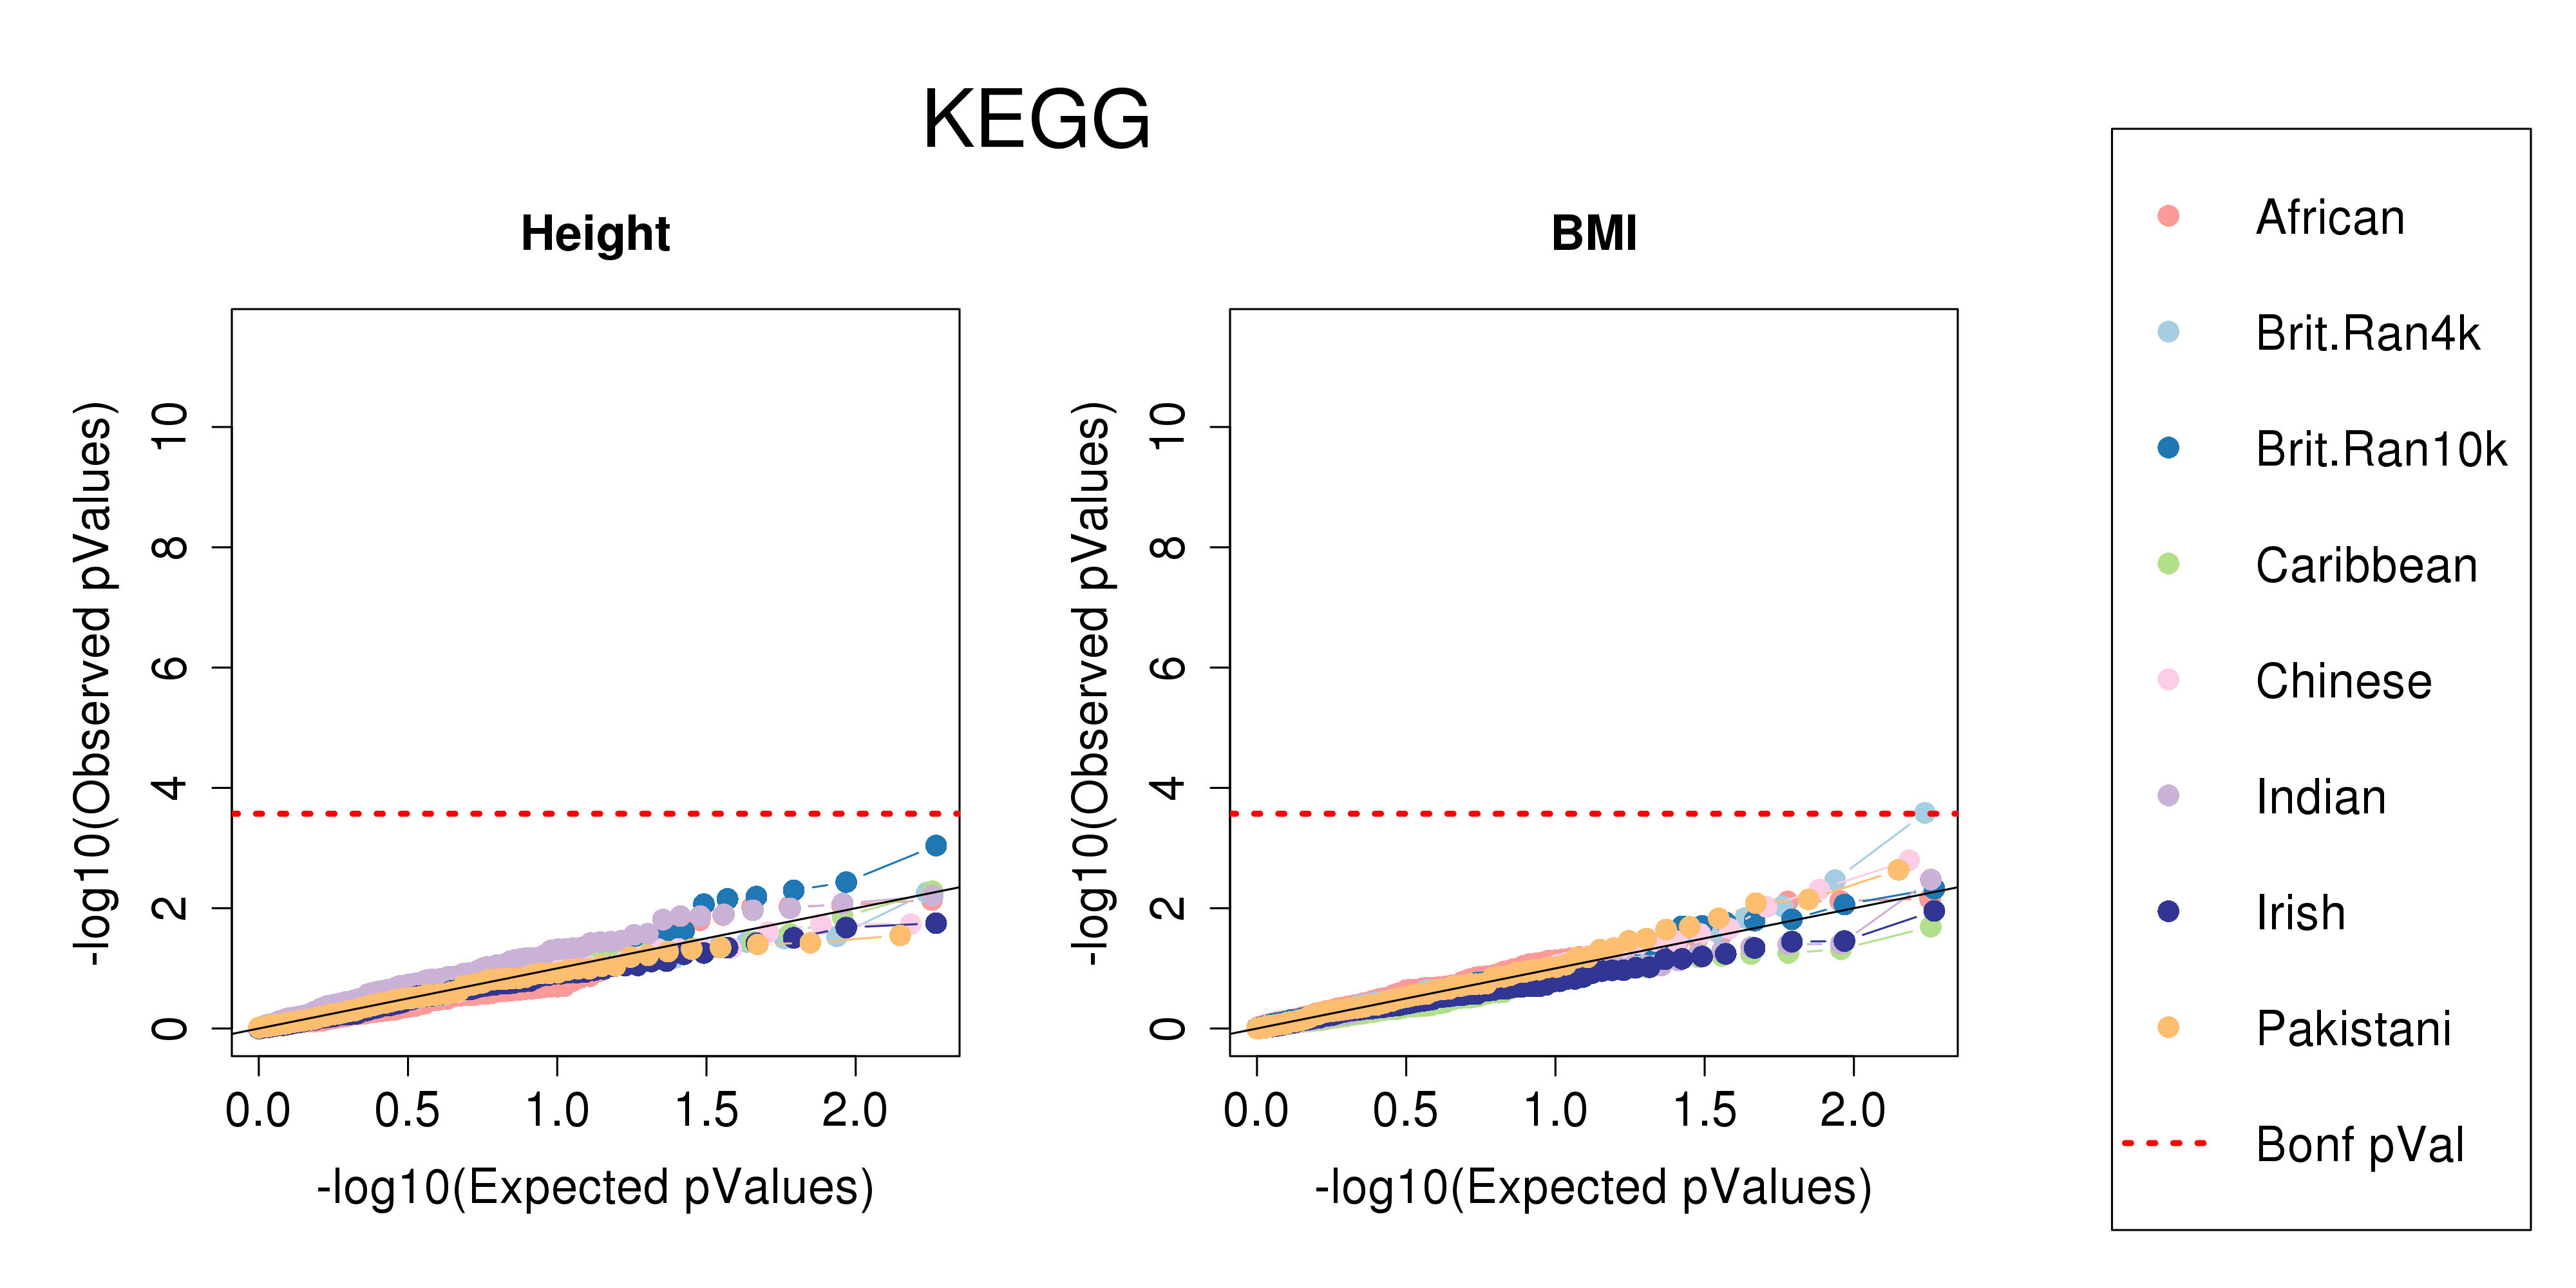
\includegraphics[scale=.35]{Images/Supp/InterPath_Supp_Figure_QQPlots_KEGG_vs1.png}
\caption[TBD]{\textbf{InterPath Phenotype Permutation QQ-Plots}. Shown are QQ-plots for running InterPath using a single, permuted version of the phenotypes for both Height and BMI with the KEGG pathways. Phenotypes were permuted within each population subset. Shown on the $x$-axis are the -$\log_{10}$ of our expected $p$-values and the on the $y$-axis are on the -$\log_{10}$ of our observed $p$-values. The dotted red line is our Bonferroni-corrected $p$-value threshold (.05 / XX KEGG pathways). We find across all population subsets that InterPath displays the null behavior as expected when using permuted phenotypes.}
\label{InterPath-Suppl-Figure-QQPlots-KEGG}
\end{figure}

\begin{figure}[htbp]
\centering
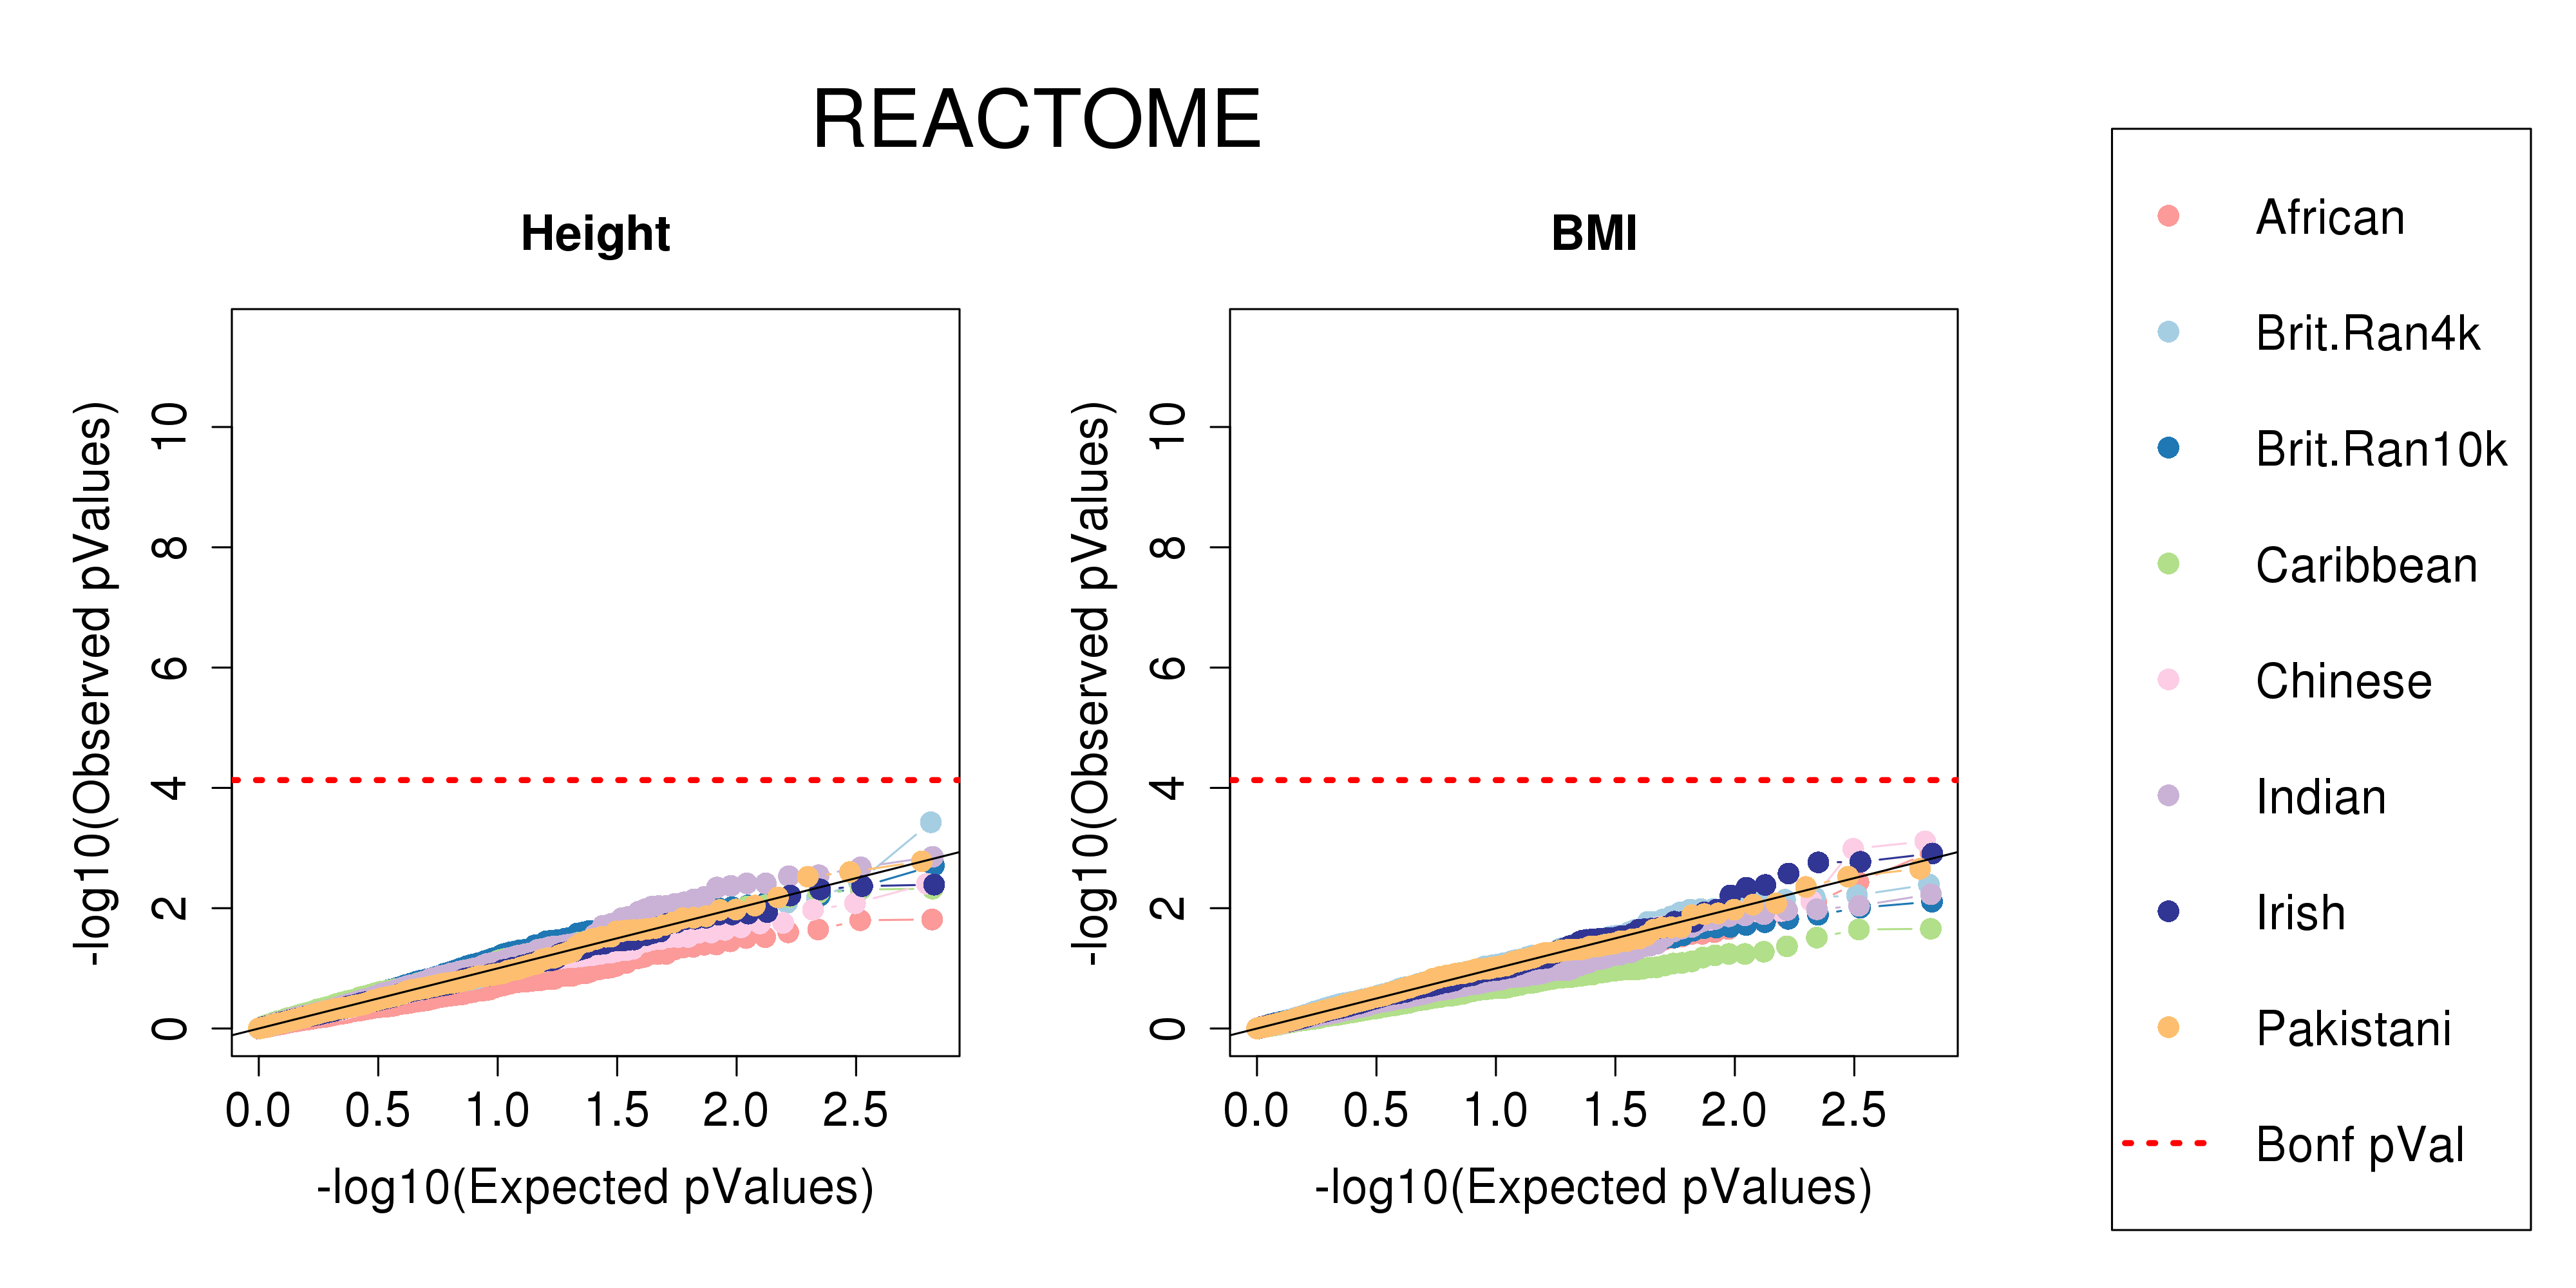
\includegraphics[scale=.35]{Images/Supp/InterPath_Supp_Figure_QQPlots_REACTOME_vs1.png}
\caption[TBD]{\textbf{TBD}. \\ Same as above (will be put in Supplementary).}
\label{InterPath-Suppl-Figure-QQPlots-REACTOME}
\end{figure}

%\begin{figure}[htbp]
%\centering
%\includegraphics[scale=.15]{Images/Supp/InterPath_Supp_pValHists_vs1.png}
%\caption[TBD]{\textbf{TBD}. \\ Placeholder.}
%\label{InterPath-Suppl-Figure-pValHists}
%\end{figure}

\begin{figure}[htbp]
\centering
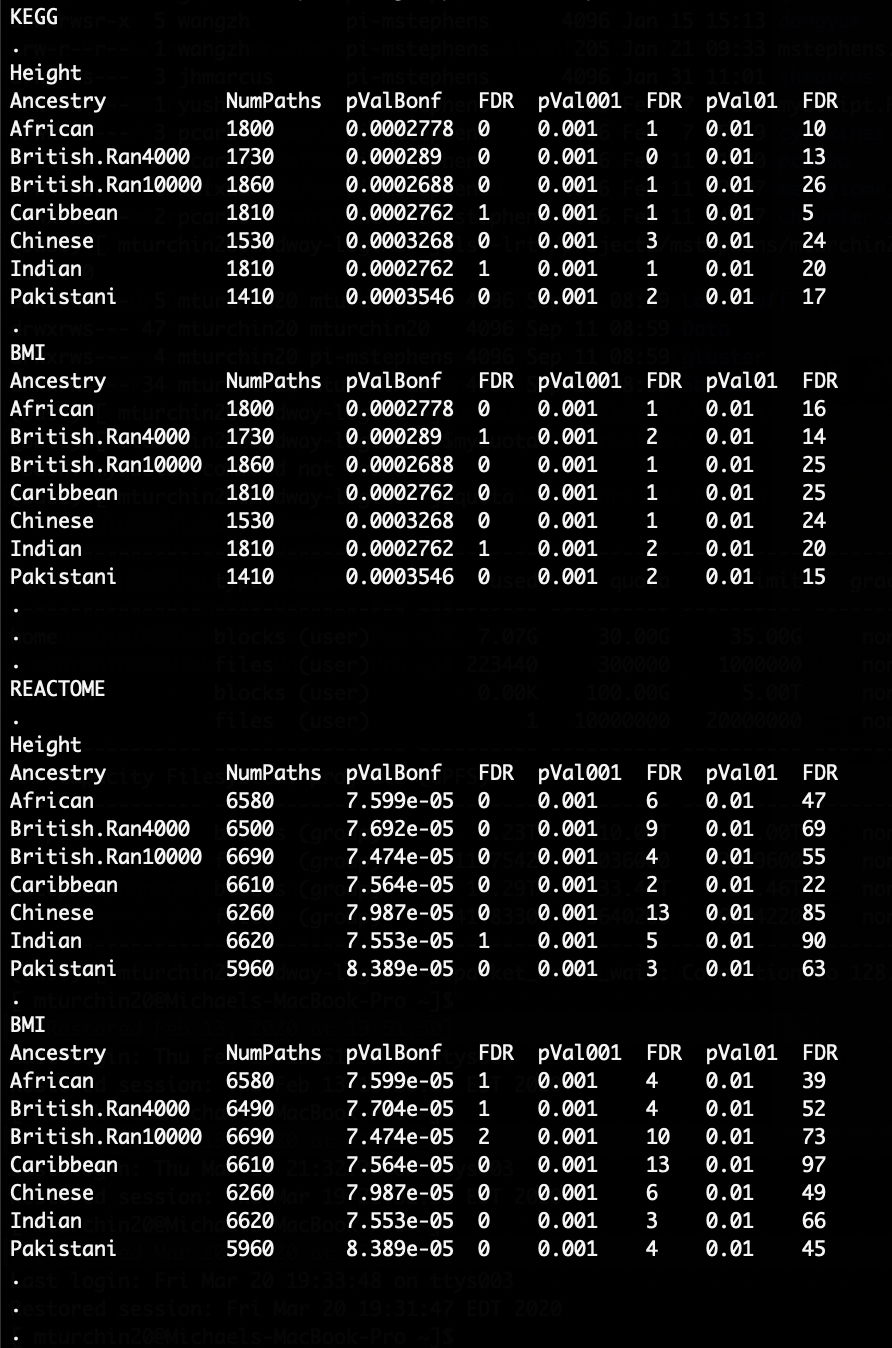
\includegraphics[scale=1.5]{Images/Supp/InterPath_Supp_Figure_FDRs_AllPops_vs1.png}
\caption[TBD]{\textbf{TBD}. }
\label{InterPath-Supp-Figure-FDR-AllPops}
\end{figure}

\begin{figure}[htbp]
\centering
\includegraphics[scale=.15]{Images/Supp/InterPath_Supp_pValsVsNumSNPs_vs1.png}
\caption[TBD]{\textbf{InterPath $p$-values Versus Number of SNPs in a Pathway}. \\ Shown is the relationship between InterPath $p$-values and the number of SNPs found in a tested pathway across all populations in height and BMI within KEGG. Shown on the $x$-axis is the number of SNPs that were included for a given pathway and on the $y$-axis is shown that pathway's InterPath -$\log_{10}$ $p$-value. As expected, we find a generally positive relationship between these two variables -- in other words, the more SNPs that are included the more likely it is that InterPath will have a more significant $p$-value. We also find, however, that it is not simply the SNPs counts that are driving this signal; looking at this same comparison within the permuted phenotype analyses we find barely any positive relationship between SNP counts per pathway and a pathway's InterPath -$\log_{10}$ $p$-value (Supplementary Figure \ref{InterPath-Suppl-Figure-pValsVsNumSNPs-perm1}}
\label{InterPath-Suppl-Figure-pValsVsNumSNPs}
\end{figure}

%\begin{figure}[htbp]
%\centering
%\includegraphics[scale=.15]{Images/Supp/InterPath_Supp_pValsVsNumSNPs_perm1_vs1.png}
%\caption[TBD]{\textbf{InterPath $p$-values Versus Number of SNPs in a Pathway, Permuted Phenotypes}. \\ Shown is the relationship between InterPath $p$-values and the number of SNPs found in a tested pathway across all populations in permuted height and BMI within KEGG. Shown on the $x$-axis is the number of SNPs that were included for a given pathway and on the $y$-axis is shown that pathway's InterPath -$\log_{10}$ $p$-value. Unlike with the observed data (Figure \ref{InterPath-Suppl-Figure-pValsVsNumSNPs}), we do not see a relationship between the number of SNPs included in a pathway and that pathway's -$\log_{10}$ InterPath $p$-value. This shows that while having more SNPs allows InterPath to generate more power to detect epistatic interactions, our significant results are not due solely to having more SNPs.}
%\label{InterPath-Suppl-Figure-pValsVsNumSNPs-perm1}
%\end{figure}

\begin{figure}[htbp]
\centering
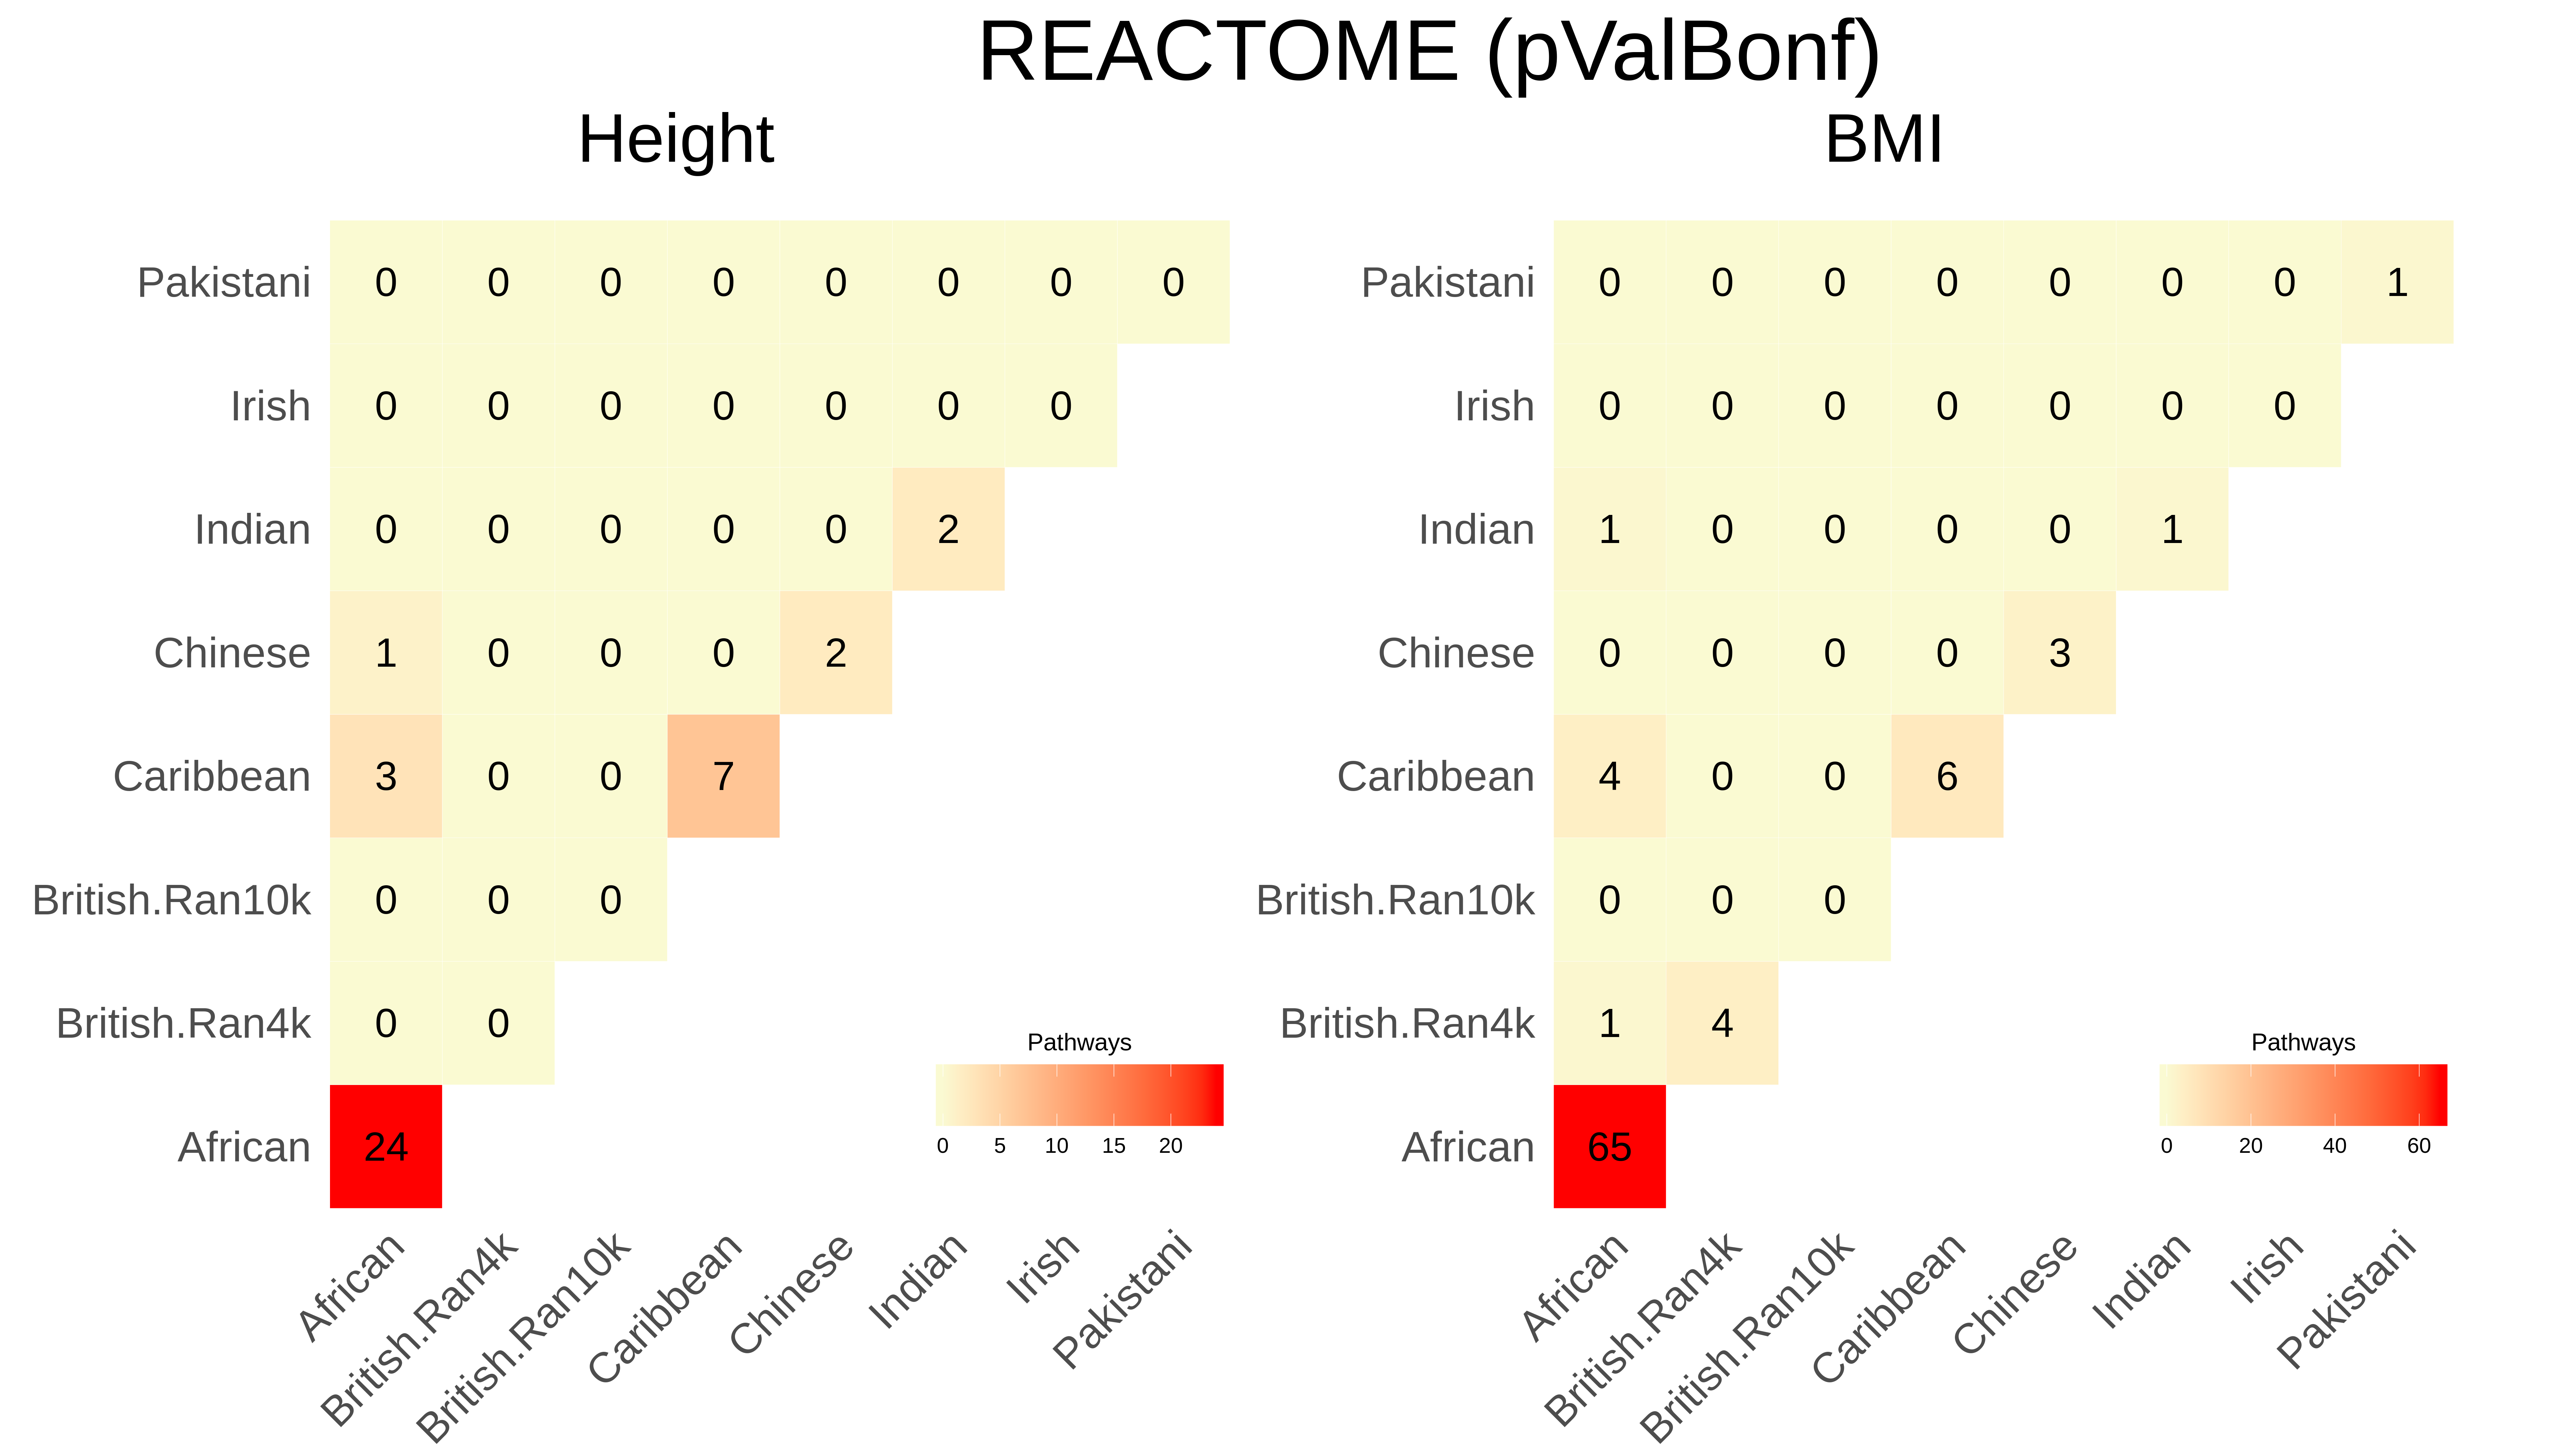
\includegraphics[scale=.225]{Images/Supp/InterPath_Supp_Figure_Heatplots_REACTOME_vs1.png}
\caption[TBD]{\textbf{TBD}. \\ See above (this would be a supplementary figure).}
\label{InterPath-Supp-Figure-Heatplots-REACTOME}
\end{figure}

\begin{figure}[htbp]
\centering
\includegraphics[scale=.15]{Images/Supp/InterPath_Supp_PhenoCompDotPlots_vs1.png}
\caption[TBD]{\textbf{InterPath Phenotype $p$-value Comparisons}. \\ Shown is a comparison of the InterPath $p$-values for both phenotypes analyzed across all population subsets in the KEGG database. Shown on the $x$-axis is the observed height -$\log_{10}$ InterPath $p$-value and shown on the $y$-axis is the observed BMI -$\log_{10}$ InterPath $p$-value. Dotted red lines represent Bonferroni-corrected $p$-value thresholds for each population/phenotype combination (.05 / number of KEGG pathways analyzed). In general we observe a correlation between InterPath $p$-values between each phenotype. In the African subset, where we have the most observed power, we find pathways that are significant in both phenotypes as well as each phenotype separately. Additionally, we observe, among marginally significant pathways, stronger InterPath signals in BMI than height -- this is in line with previous observations that BMI may contain higher levels of epistasis than height (citations).}
\label{InterPath-Suppl-Figure-PhenoCompDotPlots}
\end{figure}

\begin{figure}[htbp]
\centering
\includegraphics[scale=.35]{Images/Supp/InterPath_Supp_Figure_IBS_AllPops_vs1.png}
\caption[TBD]{\textbf{IBS Proportions vs. InterPath $p$-values in All UKB Subsets}}
\label{InterPath-Supp-Figure-IBS-AllPops}
\end{figure}

\section{Supplementary Tables}\label{Supplementary-Tables}




\begingroup
\bibliographystyle{apalike}
\setstretch{1.0}
\bibliography{Main}
\endgroup

\end{document}
